\section{Implementazione}

\subsection{Diagramma delle classi}
Il diagramma illustrato in \cref{fig:class-diagram} presenta la struttura del codice del progetto. Il framework Mesa fornisce alcune classi da estendere per agevolare la scrittura del modello, permettendo di dover implementare la sola logica applicativa.

\begin{figure}[H]
    \makebox[\textwidth][c]{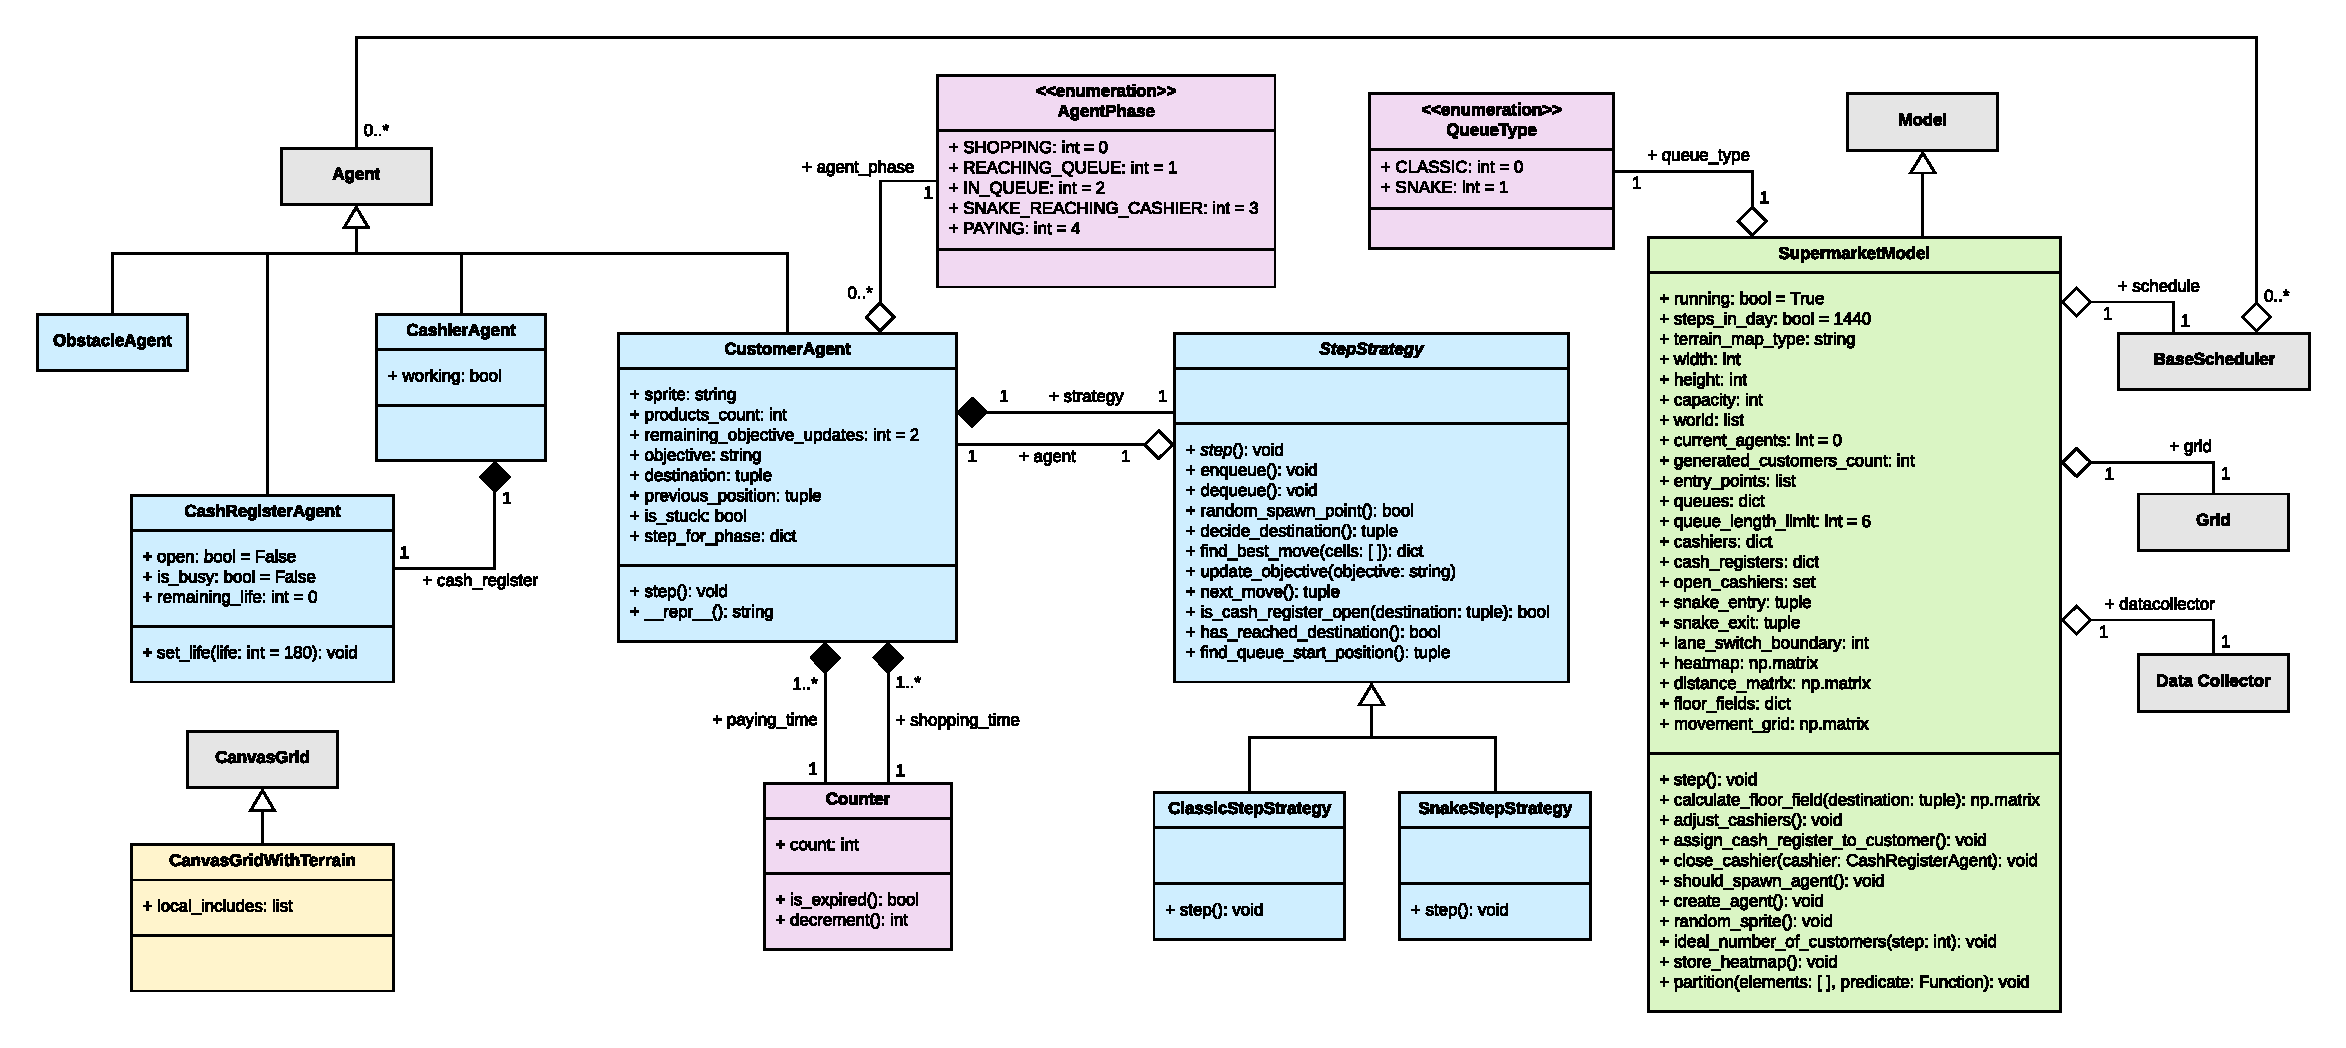
\includegraphics[width=1.45\linewidth]{class-diagram-colored.pdf}}
    \caption{Diagramma delle classi}
    \label{fig:class-diagram}
\end{figure}

\noindent
Per semplificare la comprensibilità dello schema, sono stati inclusi esclusivamente i dettagli delle classi da noi implementate, evidenziandole con colori diversi di sfondo in base alla propria finalità:
\begin{itemize}
    \item \textbf{Grigio:} classi base per permettere la simulazione di un modello attraverso Mesa.
    \item \textbf{Viola:} classi di servizio ed enumerazioni.
    \item \textbf{Azzurro:} definisce gli agenti e le strategie di movimento.
    \item \textbf{Verde:} classe principale del modello; coordina l'interazione tra Mesa e gli agenti.
    \item \textbf{Giallo:} visualizzazione e controllo dell'interazione tramite interfaccia web.
\end{itemize}

\subsection{Strategy Pattern}
La gestione di due diverse tipologie di coda, a livello implementativo, presenta molte fasi in comune, tuttavia un agente dovrà comportarsi diversamente a seconda della tipologia di coda scelta.

A tale proposito, si è scelto di implementare il pattern strategy per ridurre notevolmente la complessità del codice, evitando frequenti controlli rispetto al tipo di coda per determinare il comportamento da attuare.
